\section{Merging 3D Maps and Atomic Structures: Rigid Fitting}
Once we have the predicted \ttt{model} of any structural element included in our map, to fit that \ttt{model} in the volume constitutes the next step in the modeling workflow. Two protocols have been included in \scipion with this purpose, \scommand{powerfit} (Appendix \ref{app:powerfitProtocol}, \citep{vanzundert2016}) and \scommand{chimera rigid fit} (Appendix \ref{app:chimeraRigidFit}). The first one allows automatic fitting of models in maps, while the second one only does it when model and map are quite close, thus requiring manual fitting in advance. Although there is no a general rule to fit map and model, because it will depend on the particular problem and on our previous knowledge, in this tutorial we are going to use \powerfit application first, followed by the final \ttt{Fit in Map} in \chimera \ttt{rigid fit}. In our experience \powerfit performance decays for large 3D maps or when fitting atomic models that cover a small region of the 3D map.

\subsection*{Initial rigid fit with \powerfit}
 Open \scommand{powerfit} protocol ((\ffigure{fig:powerfit_protocol} (1)), and complete the form with the \iii{model} of atomic structure previously saved in \chimera (2), the extracted unit cell volume (3), and volume resolution (4). Among the advanced parameters, consider carefully the angular step (5) according to the size of your volume and your computing power. Despite getting a more accurate result, fitting of large volumes takes more time as  lower values of angular step are requested.  
 
 \begin{figure}[H]
  \centering 
  \captionsetup{width=.7\linewidth} 
  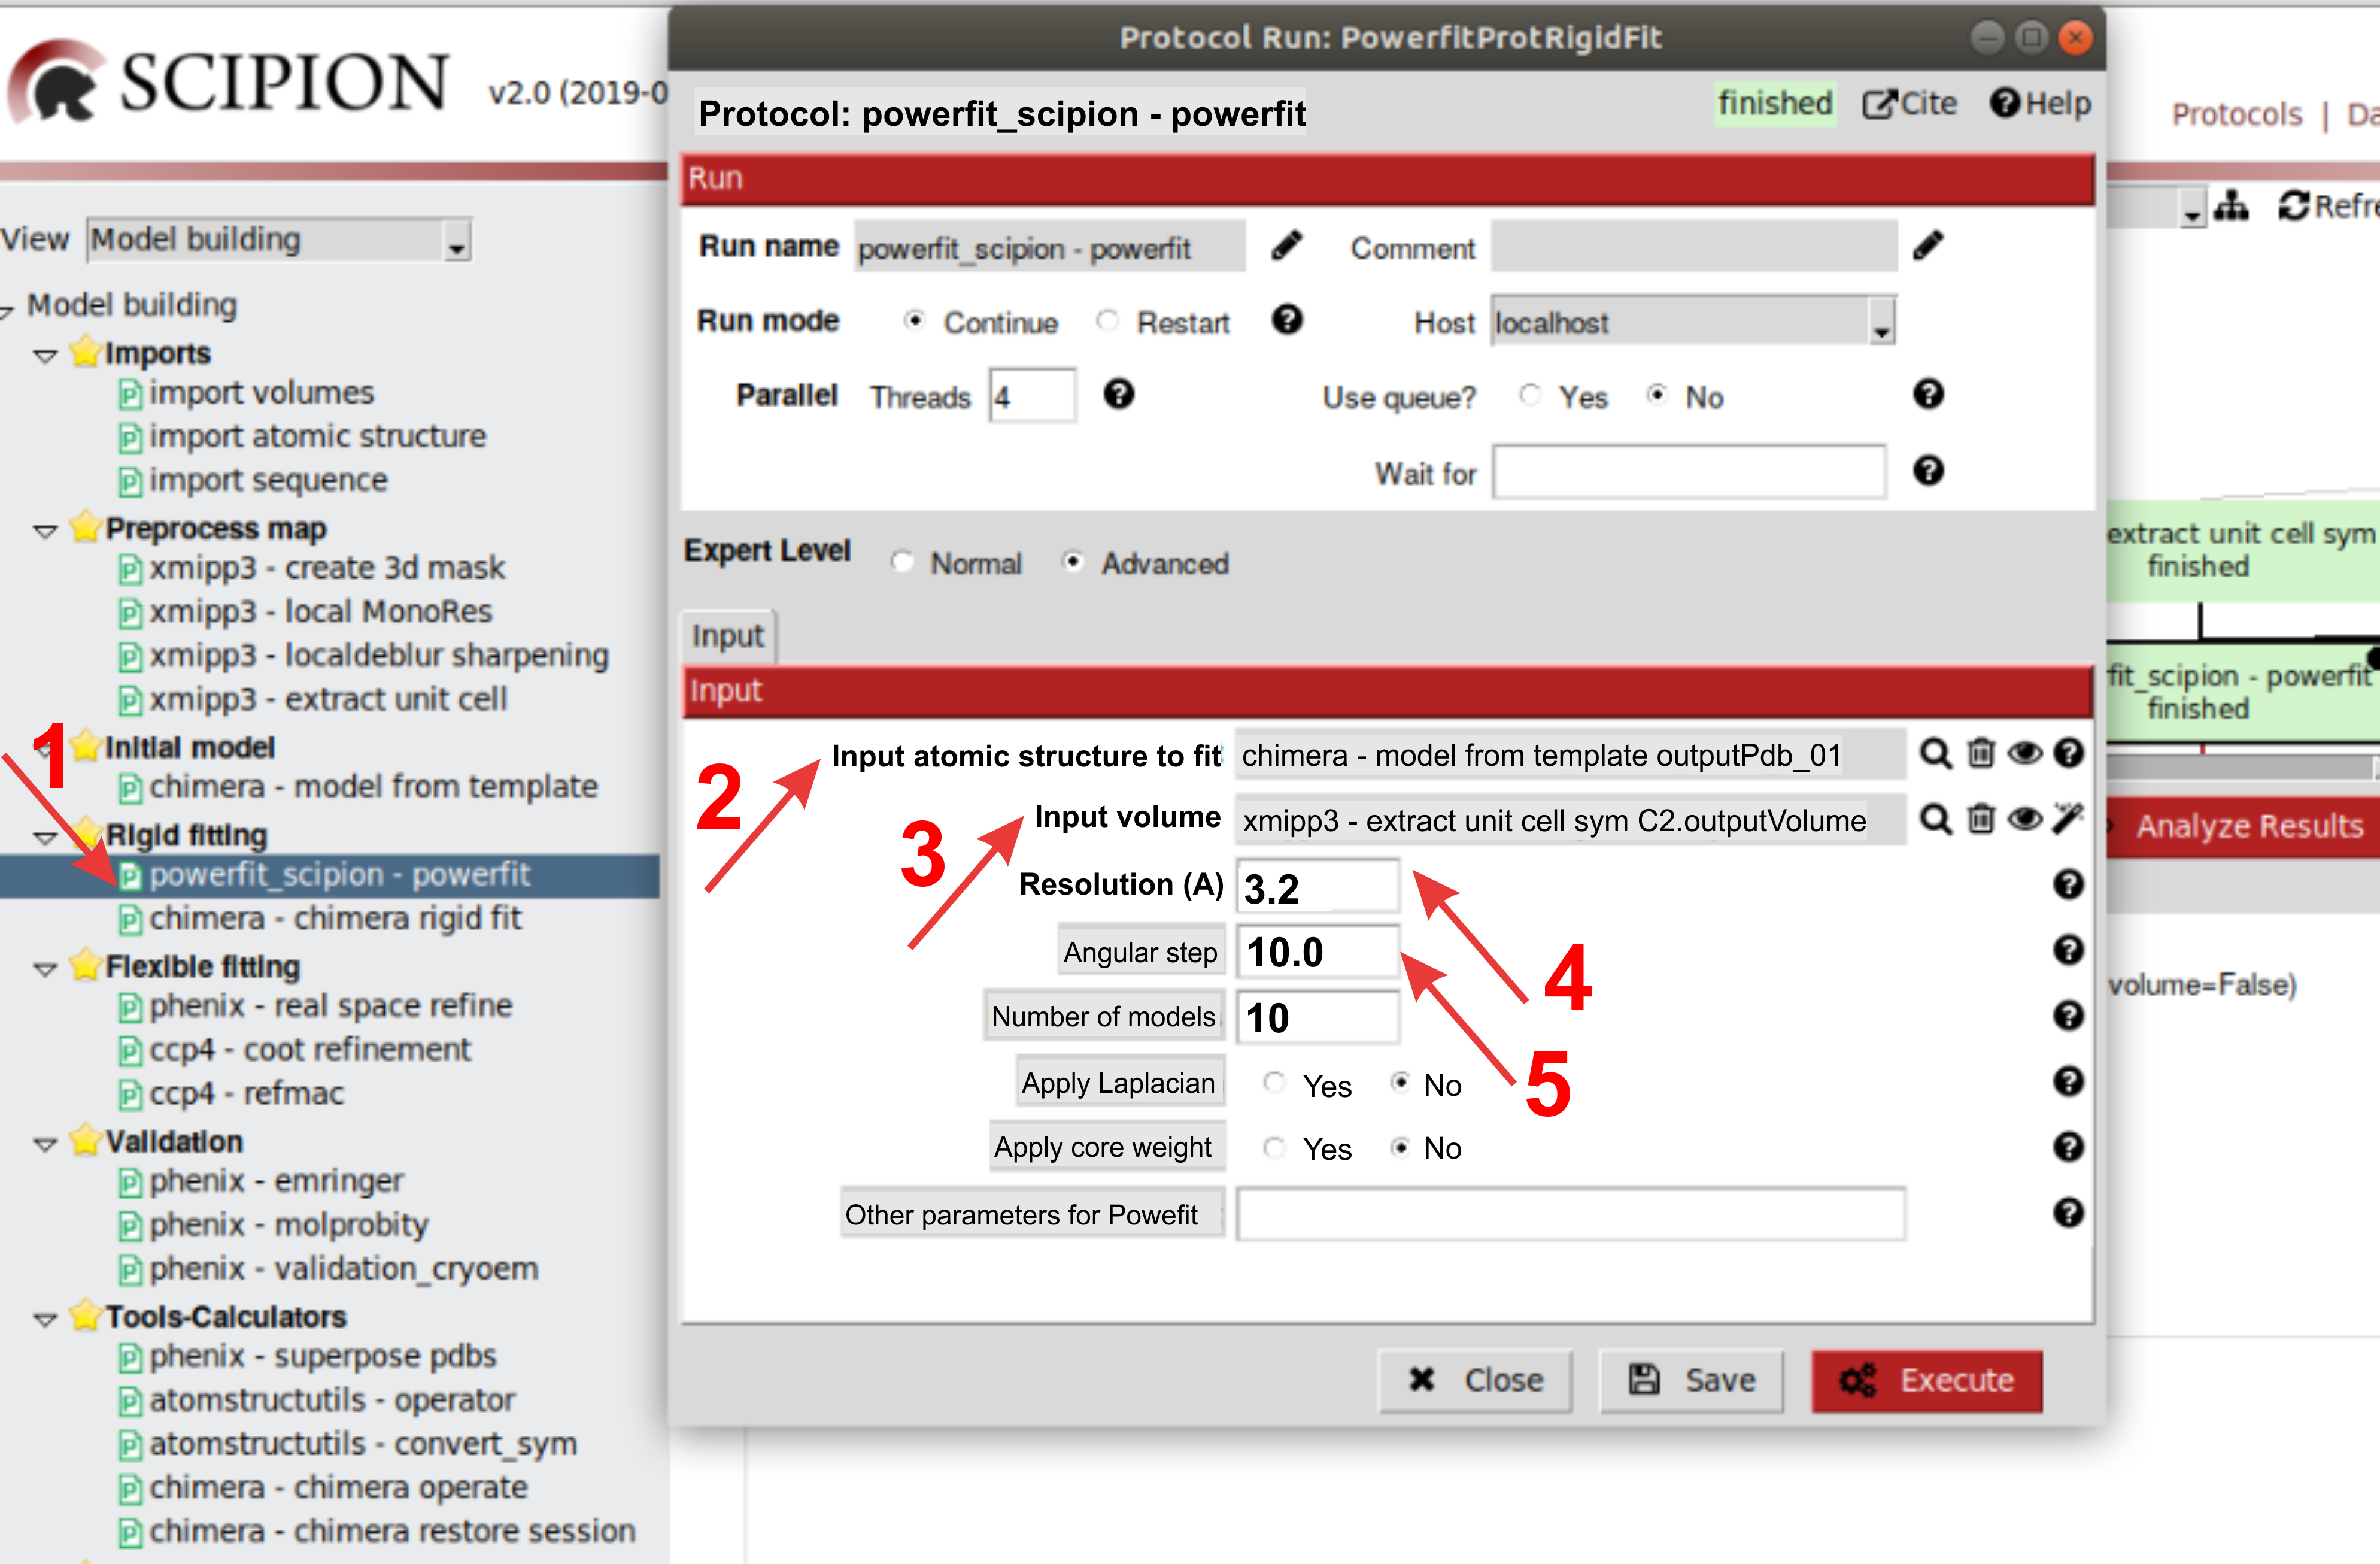
\includegraphics[width=0.85\textwidth]{Images/Fig18}
  \caption{Rigid fit with \powerfit: Filling in the protocol form.}
  \label{fig:powerfit_protocol}
  \end{figure}
 
 After executing the \scommand{powerfit} protocol, you can check results ((\ffigure{fig:powerfit_results_table} (A)(1)). The first table opened allows you to check the fitting quality (2) of best score-ordered fits in a second table (B). In our example only two fits are proposed. You can check which one fits better to the map by writing the selected fit number in the \ttt{Model to visualize} square window, and then displaying the fitting (3).
 
 \begin{figure}[H]
  \centering 
  \captionsetup{width=.7\linewidth} 
  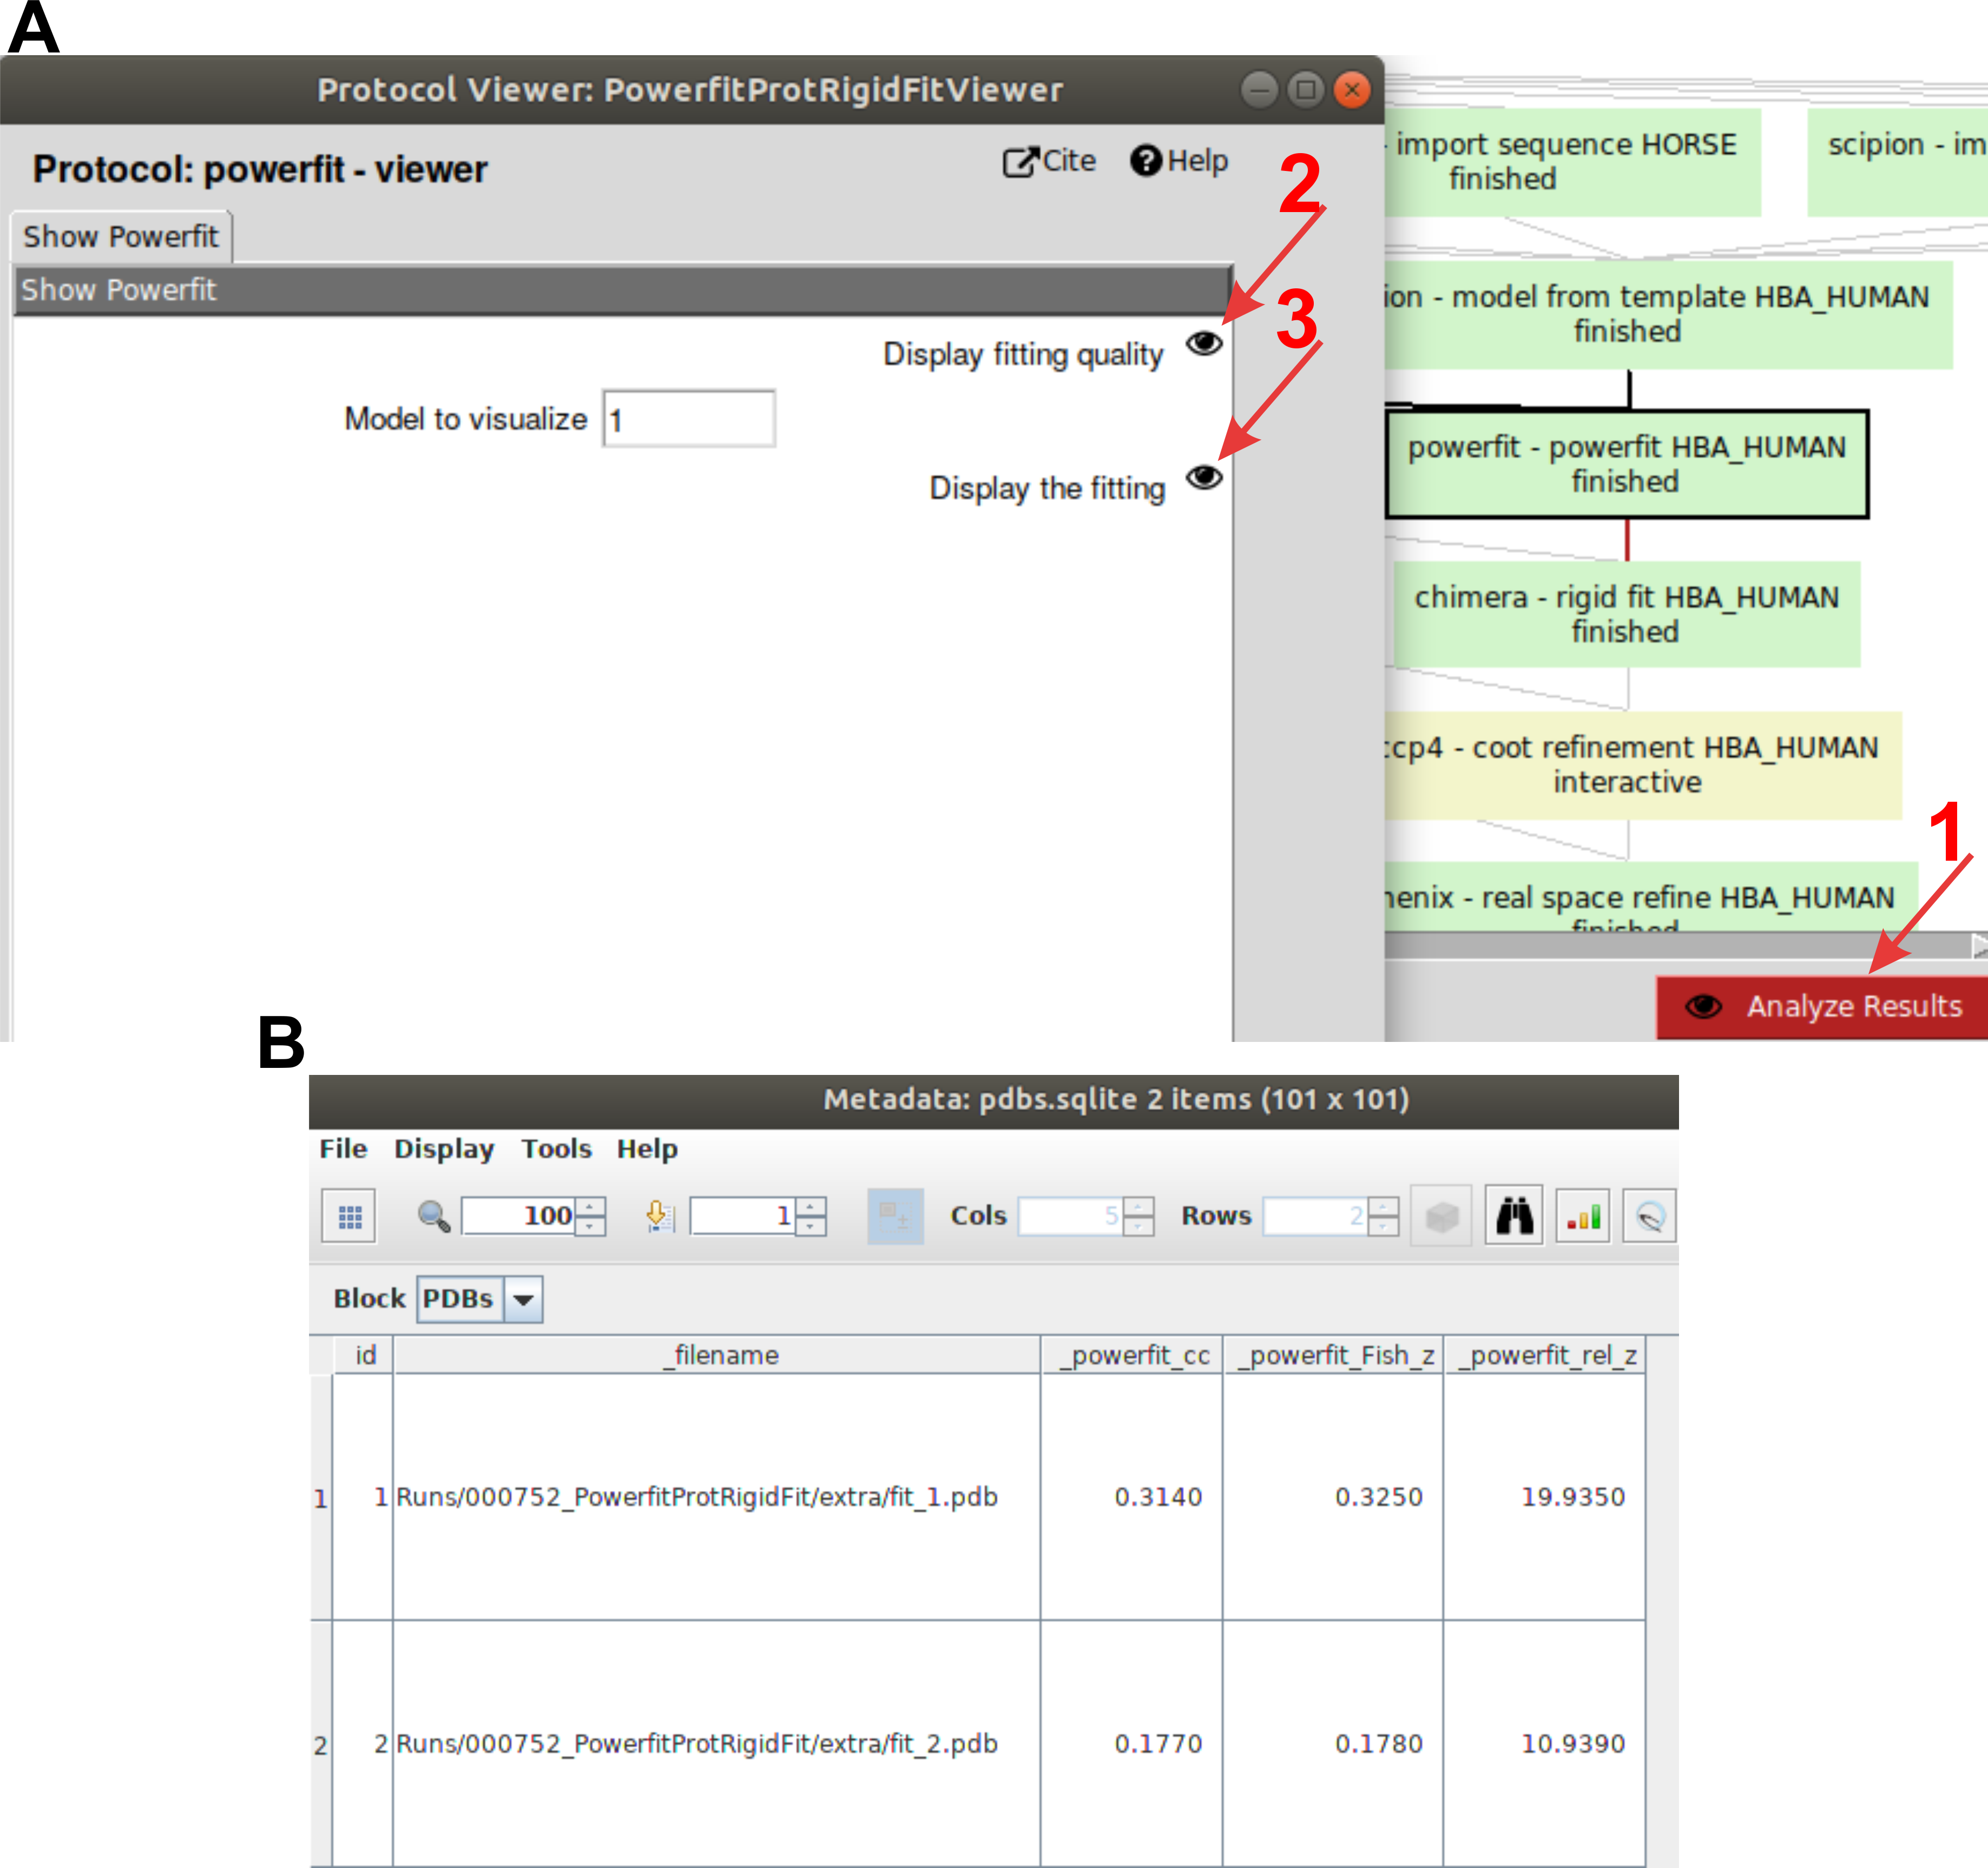
\includegraphics[width=0.85\textwidth]{Images/Fig19}
  \caption{Rigid fit with \powerfit: Checking results by score.}
  \label{fig:powerfit_results_table}
  \end{figure}
  
  \ffigure{fig:powerfit_results_figs} shows the fitting of the two possible fits between map and \ttt{models} posed by \powerfit (\ttt{fit\_1.pdb} (A), and \ttt{fit\_2.pdb} (B), green- and pink-colored, respectively). Although both of them seem to fit quite well the extracted unit cell map, only one of them should be OK. The other $model$ one must misfit the volume area that corresponds to \ttt{metHgb} $\beta$ subunit. This anomalous behavior of our \iii{model} is not surprising because \ttt{Hgb} $\alpha$ an $\beta$ subunits are 42.86\% sequence identical. 
  
 \begin{figure}[H]
  \centering 
  \captionsetup{width=.7\linewidth} 
  \includegraphics[width=0.85\textwidth]{Images/Fig20}
  \caption{Rigid fit with \powerfit: Checking the best fits in \chimera.}
  \label{fig:powerfit_results_figs}
  \end{figure}
  
 \subsection*{ Completing rigid fit with \chimera \ttt{rigid fit}}
 
 In order to assess which one of the structures fits the map better, the fitting has to be improved with \scommand{chimera rigid fit} protocol. Open this protocol (\ffigure{fig:chimera_rigid_fit} (1)), include the extracted unit cell as volume (2), one of the structure fits previously obtained with \powerfit (3), the other one (4), and execute the protocol.
 
 \begin{figure}[H]
  \centering 
  \captionsetup{width=.7\linewidth} 
  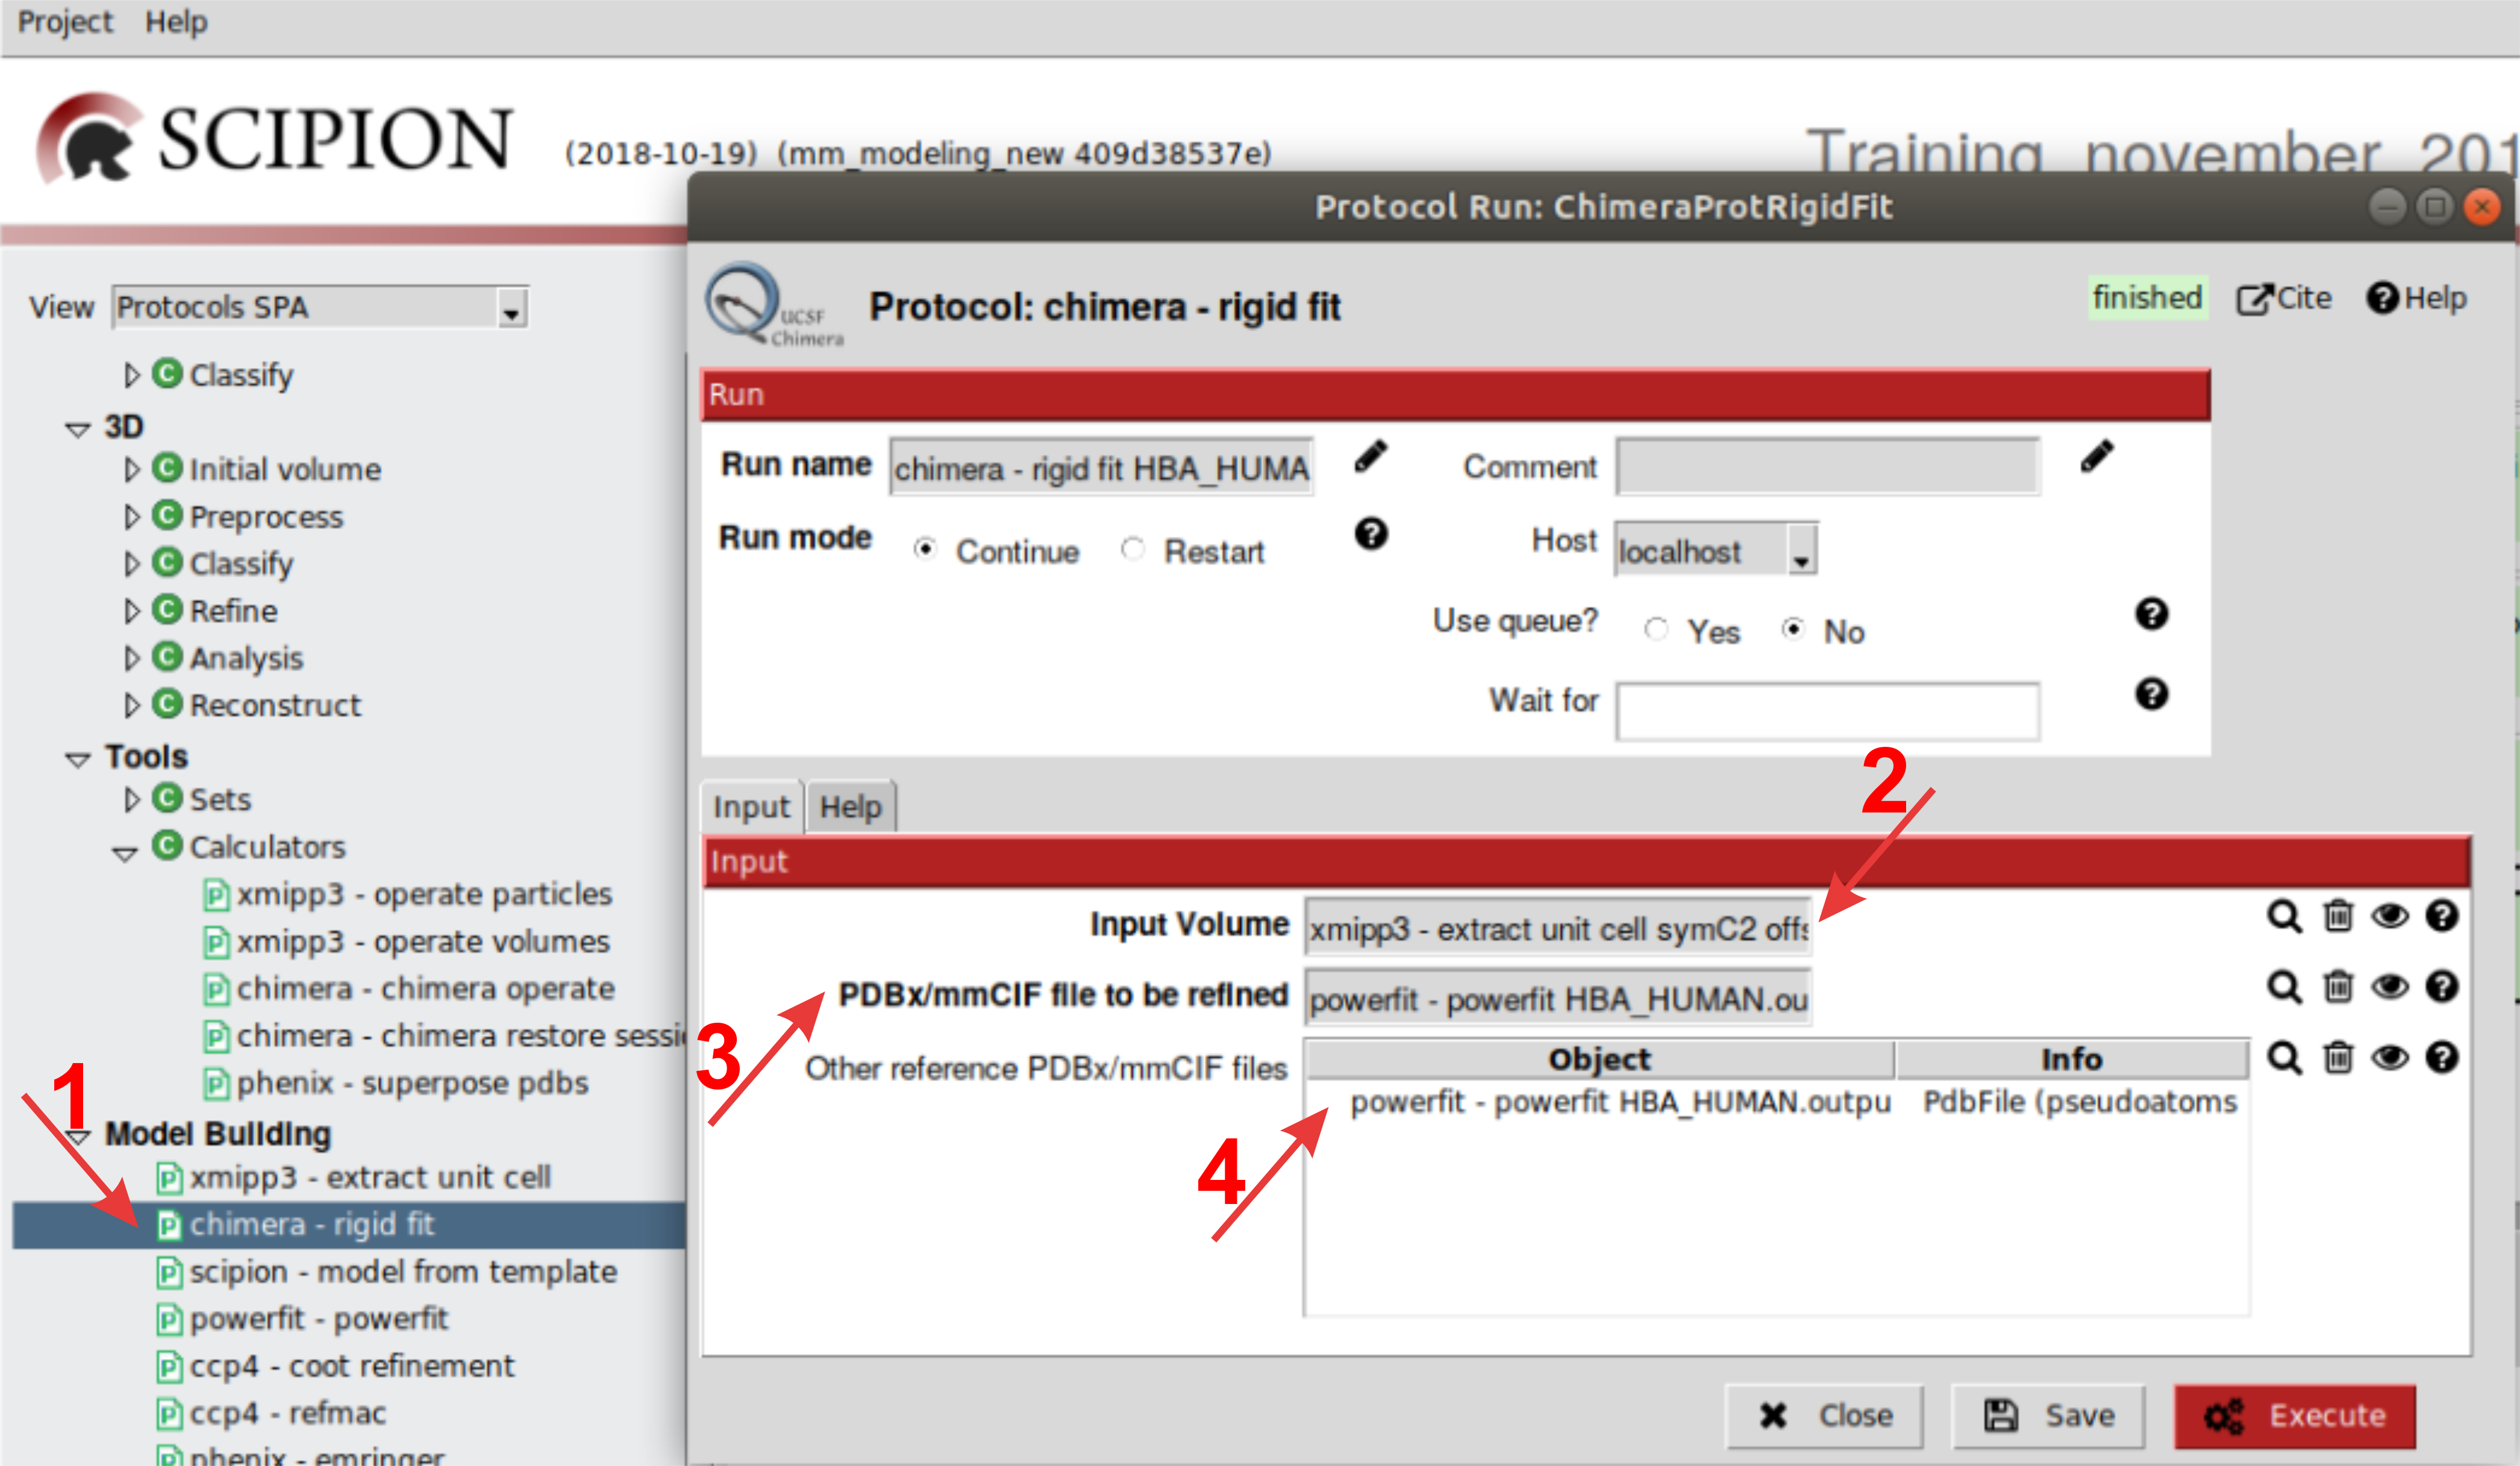
\includegraphics[width=0.85\textwidth]{Images/Fig21}
  \caption{Completing the \chimera rigid fit protocol form.}
  \label{fig:chimera_rigid_fit}
  \end{figure}
  
  Once opened \chimera graphical window, select in the upper main menu \ttt{Tools -> Volume Data -> Fit in Map}. A small window will be opened. Select each one of the fits in \ttt{Fit} and press \ttt{Fit} to allow the automatic rigid fitting. At the lower right side of \ffigure{fig:chimera_fit_in_map}, respective windows of \ttt{Fit in map} for \ttt{fit\_1.pdb} and \ttt{fit\_2.pdb} are detailed. In spite that the amount of \ttt{atoms outside the contour} is higher in \ttt{fit\_1.pdb} than in \ttt{fit\_2.pdb}, we can not conclude that the second fitting is better than the first one, because the \ttt{Average map value} is also lower. Visual inspection of both fits should identify the appropriate fitting of \iii{model} in map.
  
  \begin{figure}[H]
  \centering 
  \captionsetup{width=.7\linewidth} 
  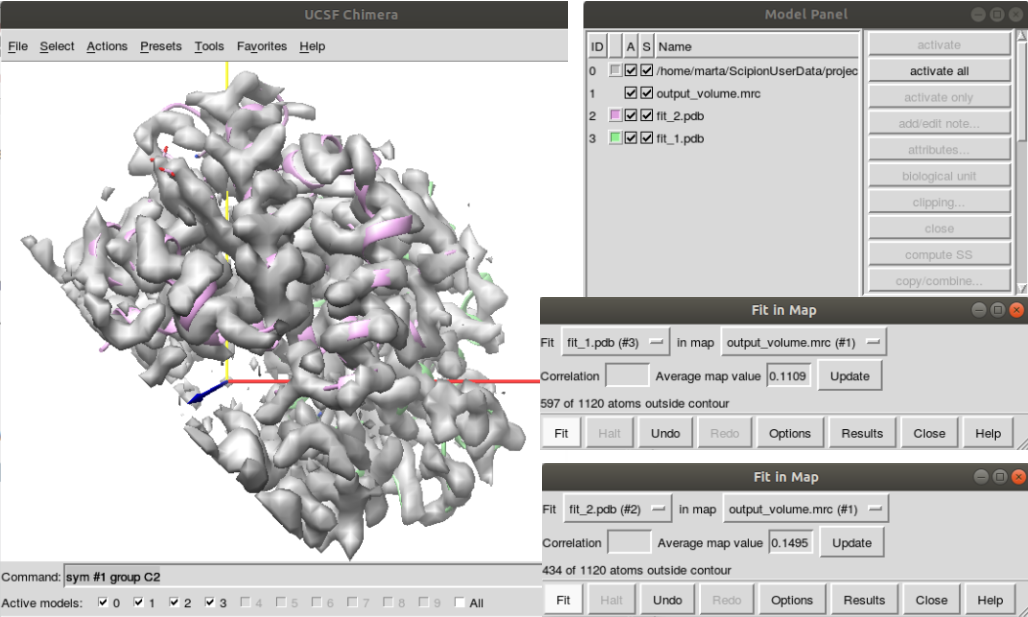
\includegraphics[width=0.85\textwidth]{Images/Fig22}
  \caption{Fitting in map with \chimera.}
  \label{fig:chimera_fit_in_map}
  \end{figure}
   
  As suggestion, before starting the visual inspection in \chimera, check first the parts of the structure that could differ the most between \ttt{metHgb} $\alpha$ and $\beta$ subunits. These divergent parts can be identified by performing an additional alignment including the $\beta$ subunit sequence. Possible steps to perform this multiple alignment: (1) import the  \ttt{metHgb} $\beta$ sequence (UnitProt id=P68871), (2) copy the protocol \scommand{model from template} and (3) add the  \ttt{metHgb} $\beta$ in the field \ttt{other sequences to align}. \ffigure{fig:multiple_alignment_HBB} shows the result of incorporating the $\beta$ subunit sequence (in yellow) to the alignment shown in \ffigure{fig:chimera_alignment}. Two regions that contain gaps of sequence are remarked in red frames. The first one, involving residues 19 and 20, absent in $\beta$ subunit, and the second one, after residue 51, could be the most relevant to differentiate between subunits. Look at them and identify the correct fit. You can highlight those residues in \chimera writing in the command line:\\
  \ttt{sel :19-20}\\
  \ttt{sel :50-55}
  
  \begin{figure}[H]
  \centering 
  \captionsetup{width=.7\linewidth} 
  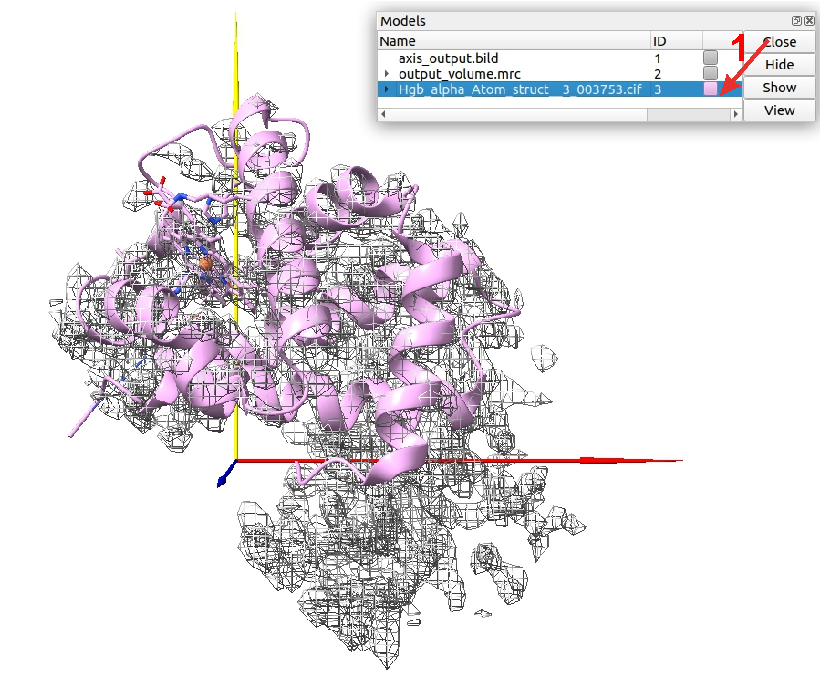
\includegraphics[width=0.85\textwidth]{Images/Fig23}
  \caption{Multiple sequence alignment including \ttt{Hgb} $\beta$ subunit (\ttt{HBB\_HUMAN}).}
  \label{fig:multiple_alignment_HBB}
  \end{figure}
  
  Once identified the appropriate fit, you can save it as fitted $model$ of the \ttt{metHgb} $\alpha$ subunit. Replacing \ttt{n} by your $model$ number (\ttt{1}, \ttt{2}), write in the command line of \chimera graphical window:\\
  
  \ttt{scipionwrite model \#n refmodel \#1 saverefmodel 0}\\
  
In case you are still unable to decide which one is the best fit, don't worry. You will make your mind up with the next step in the workflow, but then save both fits with \ttt{scipionwrite} \chimera command line. Don't forget to change the $model$ number. Your fitted models will be saved by \chimera with names \ttt{chimeraOut0001.pdb} and \ttt{chimeraOut0002.pdb}.
 
